% =====================================================================
% MARSA: Multi-accent Audio Recordings for Spanish Anti-spoofing
% Data Descriptor manuscript. Target venue: Scientific Data (Nature).
%
% SELF-CONTAINED single file: the bibliography is embedded below as a
% manual thebibliography environment, so this compiles in Overleaf with
% ONE paste and ONE run of pdflatex (no bibtex/biber step required).
%
% Structure follows the Scientific Data Data Descriptor template:
%   Background & Summary / Methods / Data Records / Technical Validation
%   / Usage Notes / Code Availability / Data Availability.
%
% Items still genuinely OUTSTANDING are flagged inline with the macro
% \PENDING{...} (rendered in red). They are NOT done. As of 2026-07-09:
%   - Author list and affiliations
%   - Baseline anti-spoofing EER (Technical Validation)
%   - Chatterbox / OuteTTS acoustic-quality metrics (WER/NISQA/SIM)
%   - Zenodo deposit DOI
% =====================================================================
\documentclass[11pt]{article}

\usepackage[utf8]{inputenc}
\usepackage[T1]{fontenc}
\usepackage{lmodern}
\usepackage[margin=1in]{geometry}
\usepackage{booktabs}
\usepackage{graphicx}
\usepackage{amsmath,amssymb}
\usepackage{siunitx}
\usepackage{multirow}
\usepackage{array}
\usepackage{xcolor}
\usepackage{tikz}
\usetikzlibrary{arrows.meta,positioning,fit,backgrounds}
\usepackage[colorlinks=true,linkcolor=black,citecolor=black,urlcolor=blue]{hyperref}
\usepackage{xurl}
\usepackage[numbers,sort&compress]{natbib}
\bibliographystyle{unsrtnat}

% Flag for items that are genuinely not finished yet.
\newcommand{\PENDING}[1]{\textcolor{red}{\textbf{[PENDING: #1]}}}

\title{\textbf{MARSA: A Multi-accent Corpus of Full and
Partial Voice Spoofing Attacks for Spanish Anti-spoofing Research}}

\author{%
Tom\'as Acosta Bernal$^{1}$, Juan Camilo V\'asquez Correa$^{2}$,
Mart\'in Daniel Calder\'on Acosta$^{1}$,\\
Rub\'en Francisco Manrique$^{1,\ast}$ \\[4pt]
\small $^{1}$Universidad de los Andes, Bogot\'a, Colombia \\
\small $^{2}$Vicomtech Foundation, Basque Research and Technology Alliance (BRTA), Donostia - San Sebastián, Spain \\
\small $^{\ast}$Corresponding author: \PENDING{email}
}
\date{}

\begin{document}
\maketitle

% =====================================================================
\begin{abstract}
\noindent
Neural text-to-speech (TTS) and voice-cloning technology increasingly
enable voice-based fraud, impersonation, and disinformation, extending
well beyond defeating automatic speaker verification (ASV) systems. The
same technology drives identity theft, fraudulent phone calls that
impersonate a trusted contact, fabricated audio misattributed to public
figures, and cloned voice messages circulated on messaging platforms. However, the datasets used to build and benchmark spoofing countermeasures
are predominantly English or Mandarin, whereas Spanish (the world's second
most-spoken native language, with approximately 485 million native
speakers \citep{ethnologue2025} distributed across two continents and
numerous mutually intelligible but acoustically distinct varieties) has
had no large-scale, openly available anti-spoofing corpus that captures
both full-utterance synthesis and partial (word-level) manipulation. We introduced \textbf{MARSA} (Multi-accent Audio Recordings for Spanish
Anti-spoofing), a corpus of 240{,}995 utterances built
from 35{,}927 bonafide recordings spanning seven Spanish accents across
Spain and Latin America. MARSA comprises three tiers. The first tier holds 186{,}647 full-spoof
utterances generated by six state-of-the-art open TTS voice-cloning
systems. The second tier holds 18{,}421 partial-spoof utterances, in
which one to three words of an otherwise bonafide recording are replaced
by cloned speech using an energy-aware splicing engine with seven fade
techniques and an optional boundary-homogenization variant that removes
a known detector shortcut. The third tier is an
acoustic-augmentation layer (reverberation, additive noise, and telephony/VoIP codecs, applied
singly and in stacked combination) at four multiplicative factors. All data is released in the ASVspoof2019 Logical Access protocol format, including frame-level spoof labels for the partial spoof tier, as well as system-level identifiers that link each spoofed utterance to its generating algorithm and, for partial spoof samples, to the corresponding replacement tier and splice variant. These identifiers give MARSA
support for multi-class attack-type attribution and source-tracing
identification in addition to bonafide vs. spoof detection, for
cross-condition benchmarking of Spanish anti-spoofing detectors, and,
more broadly, for studying how language and dialect affect the
generalization of spoofing countermeasures.
\end{abstract}

% =====================================================================
\section*{Background \& Summary}

Voice cloning is not solely a threat to biometric authentication. The same underlying technology enables identity theft and impersonation of private individuals, fabricated audio misattributed to public figures for disinformation and fake news, fraudulent phone calls that impersonate a trusted contact to extract money or information \citep{forbes2019ceofraud,destefano2023testimony,europol2022deepfakes}, and cloned voice messages circulated on messaging platforms \citep{infobae2026whatsapp}. These threats are especially well documented in Latin America, where official police statistics and journalistic reporting describe a rising pattern of voice-cloning extortion and family-impersonation scams \citep{infobae2025colombia,infobae2026whatsapp}. The damage extends beyond cases where a listener is actively deceived. A large-scale listening study spanning 35{,}532 human judgments across 138 synthesis systems found that, as synthetic speech has improved, human accuracy at correctly identifying genuine recordings fell sharply (72.7\% to 64.1\%) while accuracy at catching fakes stayed comparatively stable (72.9\% to 71.2\%). This erosion of trust in authentic audio compounds the direct fraud risk \citep{muller2026erodingtrust}.

Automatic Speaker Verification (ASV) bypass is nonetheless the best-studied instance of this threat, because it is the one setting with standardized, large-scale benchmarks. A related line of work, Spoofing-Aware Speaker Verification (SASV), jointly optimizes speaker verification and spoof detection rather than treating them as independent subsystems \citep{sasvevalplan2022,sasv2022}. The underlying synthesis technology and the countermeasures needed to detect it are shared across all of these settings. A corpus built for ASV-focused detection therefore transfers directly to detecting synthetic or manipulated speech in these other, non-biometric contexts.

Within this broader threat landscape, this Descriptor focuses on ASV, which is deployed at scale for authentication in banking, telephony, and access control. Its principal security threat is voice spoofing, in which an attacker synthesizes or clones a target speaker's voice to defeat the verifier. The ASVspoof challenge series established the standard datasets and evaluation protocols for this problem \citep{asvspoof2019,asvspoof2021,asvspoof5}, and a large body of work has since developed neural countermeasures such as RawNet2, wav2vec\,2.0 front-ends, and graph-attention detectors \citep{rawnet2,tak2022ssl,aasist}. More recent work has moved toward larger self-supervised backbones and dedicated benchmarking infrastructure for comparing them, including compact-backbone studies such as RAPTOR \citep{raptor2026} and the Speech DF Arena leaderboard \citep{dowerah2025speechdfarena}.

This body of work almost universally casts the problem as binary detection (bonafide vs.\ spoof). Once a signal is flagged as spoofed, identifying which generation algorithm produced it is rarely addressed. Attack-type attribution matters for the forensic response and for tracking which synthesis methods are actively being weaponized. Datasets built around a single generation family, most notably ASVspoof2019 itself \citep{asvspoof2019}, already assign a system-level label to each full-utterance attack, but this granularity has not extended to partial, word-level splices, where the generating system, replacement tier, and splice technique of each edit are rarely all recorded together. MARSA's protocol format encodes this information for every spoofed utterance, full or partial (Data Records), extending multi-class attack-type classification to the partial-spoof setting alongside standard binary detection.

A recurring and well-documented failure of these countermeasures is poor generalization. A detector that performs near-perfectly on its training distribution degrades sharply on unseen synthesis systems, recording conditions, or corpora \citep{muller2022generalize,muller2024harder}.

The datasets that anchor this research are, with few exceptions, English (the ASVspoof Logical Access sets derive from English source speech) or Mandarin (the Half-Truth partial-fake corpus \citep{yi2021had}). Recent large multilingual corpora such as MLAAD \citep{mlaad} and SpeechFake \citep{speechfake} do include Spanish, but only as one of dozens of languages, with a single accent per language and without a partial-spoof or dialect-stratified design. The one dedicated Spanish resource, HISPASpoof \citep{hispaspoof}, provides real and fully synthesized speech in six accents, but is limited to full-utterance synthesis, with no partial-spoof tier, no boundary-shortcut control, and no acoustic-augmentation layer. The original HABLA dataset \citep{habla} was an early step toward Latin American Spanish anti-spoofing, but is limited in speaker count, accent coverage, and attack diversity, and does not address partial spoofing. No existing resource combines large-scale, cross-continental Spanish coverage with both full and partial spoofing and a channel-augmentation layer, which is the gap MARSA fills. Table~\ref{tab:corpuscompare} summarizes these resources side by side.

\begin{table}[t]
\centering
\caption{MARSA compared with the closest existing corpora. Full-spoof
and partial-spoof columns report utterance counts where the source
paper states them directly; MLAAD and SpeechFake report total
synthetic-audio scale across all languages rather than a Spanish-only
breakdown, since neither stratifies its Spanish portion by accent.
Aug.: dedicated acoustic-augmentation layer (reverberation, noise,
codec).}
\label{tab:corpuscompare}
\small
\begin{tabular}{lccccc}
\toprule
\textbf{Corpus} & \textbf{Accents} & \textbf{Bonafide} & \textbf{Full-spoof} & \textbf{Partial-spoof} & \textbf{Aug.} \\
\midrule
HABLA \citep{habla}      & 5 (LatAm)         & $\approx$22{,}000 & limited     & No & No \\
HISPASpoof \citep{hispaspoof} & 6 (cross-continental) & 6{,}241 & 37{,}446 & No & No \\
MLAAD \citep{mlaad}      & 1 of 54 languages & --      & \multicolumn{1}{c}{\parbox{2.1cm}{\centering 175 systems,\\1{,}003 h total}} & No & No \\
SpeechFake \citep{speechfake} & 1 of 46 languages & -- & \multicolumn{1}{c}{\parbox{2.1cm}{\centering 40 systems,\\$>$3{,}000 h total}} & No & No \\
\textbf{MARSA (this work)} & \textbf{7 (cross-continental)} & \textbf{35{,}927} & \textbf{186{,}647} & \textbf{18{,}421} & \textbf{Yes} \\
\bottomrule
\end{tabular}
\end{table}

Language is not a neutral variable for spoofing detection. Cross-dialectal acoustic variation within Spanish is large enough to degrade the performance of state-of-the-art speech models non-uniformly. Word-error rates for a single automatic speech recognition system differ by several absolute points across Argentine, Chilean, Colombian, Mexican, Peninsular, and Peruvian Spanish \citep{kantharuban2023dialectgap,nacimiento2024biases}, and Spanish varieties are separable into distinct dialect macrozones from raw acoustics alone \citep{zuluaga2023commonaccent}. A spoofing detector that must decide whether a signal is genuine (and, for partial spoofing, which segments are genuine) cannot be assumed to transfer across these varieties. Building a corpus that spans them is therefore necessary for dialect-robust Spanish anti-spoofing.

Partial spoofing---replacing a short span of an otherwise genuine utterance with synthetic speech---is a distinct and harder threat than full synthesis, because the overwhelming majority of the signal is authentic \citep{zhang2023partialspoof}, and it has been the focus of dedicated challenges such as the partially-fake track of ADD 2022 \citep{add2022}. It is also the threat for which Spanish resources are scarcest. The only existing multilingual partial-spoof benchmark that includes Spanish, HQ-MPSD \citep{li2025hqmpsd}, provides on the order of $1.3\times10^{4}$ Spanish partial-spoof utterances generated by a single TTS system from a single-accent source, with one splice method and only a single added noisy condition. Prior forensic work has further shown that partial-spoof detectors can exploit a shortcut. Because only the boundaries flanking the spliced segment are anomalous, a detector can learn to ``find the discontinuous boundary'' rather than the synthesis artifact itself, achieving low error with no training at all \citep{negroni2024splicing,huang2024detectable}. A corpus intended to drive robust detection must therefore control for this shortcut.

MARSA addresses these gaps simultaneously. Its contributions as a data resource are:
\begin{enumerate}
  \item \textbf{Scale and accent coverage.} 35{,}927 bonafide
  utterances from 1{,}567 speakers across seven Spanish accents spanning
  two continents (Peninsular Spanish and six Latin American varieties),
  paired with 186{,}647 full-spoof utterances from six independent,
  open-source neural TTS voice-cloning systems.
  \item \textbf{A diverse, richly parameterized partial-spoof tier.}
  18{,}421 partial-spoof utterances that, while comparable in scale to
  the Spanish portion of the closest prior resource, are far more
  diverse, spanning six TTS systems, seven accents, and three
  word-replacement tiers. They are built with an energy-aware splicing
  engine that varies the number of replaced words (one, two, or three),
  the acoustic placement of cuts, and the boundary fade technique, and
  that offers a boundary-homogenization variant explicitly designed to
  suppress the splice-boundary detector shortcut.
  \item \textbf{An acoustic-augmentation layer} modeling reverberation,
  environmental noise, and real telephony/VoIP codec degradation, applied
  both singly and in stacked combination at four corpus-multiplication
  factors. Channel robustness can thus be studied without regenerating
  attacks.
  \item \textbf{Attack-type attribution labels.} Every spoofed
  utterance's protocol entry identifies its specific generating system
  rather than a generic \texttt{spoof} label. Partial-spoof utterances
  additionally record their replacement tier and splice variant. MARSA
  therefore supports multi-class attack-type classification and
  attribution research, not only binary detection.
  \item \textbf{Standardized release format.} All audio follows the
  ASVspoof2019 Logical Access protocol convention, and the partial-spoof
  tier ships frame-level spoof labels. Existing anti-spoofing training
  and evaluation code can therefore consume MARSA with minimal
  adaptation.
\end{enumerate}

Table~\ref{tab:overview} summarizes the corpus. The remainder of this
Descriptor details how each tier was produced (Methods), how the release
is organized on disk (Data Records), the quality and baseline-detection
evidence that the data are fit for purpose (Technical Validation), and
practical guidance for reuse (Usage Notes).

\begin{table}[t]
\centering
\caption{MARSA corpus overview. Augmentation is released as four
separate tiers, each a full copy of the base corpus at the stated
multiplication factor (for example, the $\times$5 tier holds five times
the base utterance count and five times the base hours); a user selects
one factor rather than combining them (Usage Notes). Std.\ dur.\ is not
meaningful for the Base total row, which pools three tiers with
different duration distributions rather than describing a single one.}
\label{tab:overview}
\small
\begin{tabular}{lrrrrp{3.1cm}}
\toprule
\textbf{Tier} & \textbf{Utt.} & \textbf{Hours} & \textbf{Avg.\ dur.\ (s)} & \textbf{Std.\ dur.} & \textbf{Description} \\
\midrule
Bonafide            & 35{,}927  & 53.8  & 5.39 & 1.62  & Source corpus, 7 accents, 1{,}567 speakers \\
Full spoof          & 186{,}647 & 218.6 & 4.22 & 1.19  & 6 TTS voice-cloning systems \\
Partial spoof       & 18{,}421  & 30.2  & 5.90 & 1.61  & 1--3 word replacements (15{,}641 clean) \\
\midrule
\textbf{Base total} & \textbf{240{,}995} & \textbf{302.6} & 4.52 & --- & Pre-augmentation \\
\midrule
Augmented tiers & \multicolumn{4}{l}{$\times$2 / $\times$3 / $\times$5 / $\times$10 the base row above} & Released separately per factor \\
\bottomrule
\end{tabular}
\end{table}

% =====================================================================
\section*{Methods}

\subsection*{Bonafide source corpus}

The genuine-speech foundation of MARSA combines the original HABLA
Latin American Spanish anti-spoofing dataset \citep{habla} with
additional speakers drawn from Mozilla Common Voice \citep{commonvoice}
and added to fill the accent groups HABLA under-represents. Candidate
Common Voice speakers whose voice closely matched an existing HABLA
speaker were excluded to avoid near-duplicate voices across the two
sources; the speaker-embedding method and similarity threshold used for
this deduplication are reported in Technical Validation. Peninsular
Spanish and Mexican speakers are drawn entirely from this Common Voice
extension. Colombian and Chilean speakers are a blend of both sources.
Argentine and Peruvian speakers are unchanged from the original HABLA
release.

The bonafide data comprise 35{,}927 utterances from 1{,}567 speakers,
each labeled with one of seven accent codes. The accent distribution is
given in Table~\ref{tab:accents}. Two properties are important for
downstream use. First, the corpus is \emph{cross-continental}:
Peninsular (European) Spanish is the single largest accent group
(33.7\% of speakers), alongside six Latin American varieties. Second,
the distribution is markedly imbalanced. The three largest accents
(Peninsular, Mexican, Colombian) account for 82\% of the speakers, while
the three smallest (Argentine, Peruvian, Venezuelan) together account
for 6.6\% of speakers (Table~\ref{tab:accents}). Utterance counts do not
track this speaker imbalance. Six of the seven accents land within a
narrow band of 5{,}446--5{,}460 utterances regardless of how many
speakers contribute to that band, consistent with each accent being
built toward a roughly fixed utterance total rather than a fixed speaker
count; only Venezuelan falls well short of that band (3{,}221). The
Common Voice extension could not close that gap: its Spanish locale
contains very few self-tagged Venezuelan-accent speakers, and only one passed the
speaker-similarity filter. The group's size (23 speakers) is therefore
almost entirely inherited from the original HABLA release (22 of 23).
This imbalance is a property of the source data and is preserved, not
corrected, in MARSA, allowing users to apply their own balancing
strategy.

\begin{table}[t]
\centering
\caption{Accent composition of the bonafide source corpus. Codes: es~=~Peninsular
(Spain), mx~=~Mexican, co~=~Colombian, cl~=~Chilean, ar~=~Argentine,
pe~=~Peruvian, ve~=~Venezuelan. Speaker share is not a valid proxy for
utterance share, since utterances per speaker are not constant across
accents (Bonafide source corpus).}
\label{tab:accents}
\small
\begin{tabular}{lrrr}
\toprule
\textbf{Accent} & \textbf{Speakers} & \textbf{Utterances} & \textbf{Speaker Share} \\
\midrule
es (Peninsular, Spain) & 528 & 5{,}450 & 33.7\% \\
mx (Mexican)           & 406 & 5{,}450 & 25.9\% \\
co (Colombian)         & 357 & 5{,}450 & 22.8\% \\
cl (Chilean)           & 173 & 5{,}450 & 11.0\% \\
ar (Argentine)         & 42  & 5{,}460 & 2.7\% \\
pe (Peruvian)          & 38  & 5{,}446 & 2.4\% \\
ve (Venezuelan)        & 23  & 3{,}221 & 1.5\% \\
\midrule
\textbf{Total}         & \textbf{1{,}567} & \textbf{35{,}927} & \textbf{100\%} \\
\bottomrule
\end{tabular}
\end{table}

All audio is processed at \SI{16}{\kilo\hertz}, mono, 16-bit. Every bonafide utterance is transcribed with the Parakeet TDT multilingual transducer \citep{tdt,parakeet}, which natively emits word-level start and end timestamps through its token-and-duration architecture. Transcription accuracy is validated in Technical Validation.

A forced aligner (for example, the Montreal Forced Aligner \citep{mfa}) is not a substitute here. Forced alignment requires an independent ground-truth transcript to align against, and only the Common Voice-origin fraction of the bonafide corpus has one (Bonafide source corpus). The original HABLA recordings carry no transcript at all. Transcribing every bonafide utterance with the same method, rather than forced-aligning the Common Voice subset and transcribing the rest separately, keeps the timestamping method independent of bonafide origin and avoids a spurious cue that a detector could otherwise exploit.

Both the partial-spoof selection stage and the intelligibility metric of the quality screen draw on these word boundaries.
Utterances shorter than four words are excluded from the partial-spoof tier, because four words is the minimum sentence length at which even the smallest replacement tier can operate while keeping the spoofed fraction of the utterance below one quarter.

\subsection*{Full-spoof attack pipelines}

Each bonafide utterance is the cloning target for six independent,
open-source neural TTS voice-cloning systems, selected against four
criteria:
\begin{enumerate}
  \item \textbf{Open availability}, for reproducibility.
  \item \textbf{Demonstrated Spanish synthesis capability}.
  \item \textbf{Architectural diversity}, ensuring the corpus does not
  encode the artifacts of a single synthesis family.
  \item \textbf{Release within the 2024--2026 window}, representing
  current practice.
\end{enumerate}
The six systems are Fish-Speech \citep{fishspeech}, Qwen3-TTS
\citep{qwen3tts}, OpenVoice v2 \citep{openvoice}, Chatterbox
\citep{chatterbox}, OuteTTS \citep{outetts}, and OmniVoice
\citep{omnivoice}. They span autoregressive language-models, diffusion
language-models, and tone-conversion architectures. CosyVoice
\citep{cosyvoice} was evaluated and excluded because it produced
non-Spanish output for Spanish input text.

Table~\ref{tab:systems} summarizes the six architectures, and the
following notes give the configuration that governs each system's
artifacts.

\begin{table}[t]
\centering
\caption{Full-spoof systems: synthesis architecture, acoustic backend,
and the configuration most relevant to the artifacts each leaves in the
generated audio. \textbf{RTF}: Real-Time Factor observed on the generation
hardware (lower is faster). \textbf{LM}: Language Model}
\label{tab:systems}
\small
\begin{tabular}{p{2.1cm}p{3.0cm}p{4.6cm}}
\toprule
\textbf{System} & \textbf{Synthesis architecture} & \textbf{Backend and notable configuration} \\
\midrule
Fish-Speech & Dual autoregressive LM ($\approx$4\,B params) & Firefly-GAN decoder; served over an HTTP API; \SI{15}{\second} concatenated reference; $\approx$20\,k\,h Spanish training \\
Qwen3-TTS & Autoregressive LM & Speaker-embedding (x-vector) conditioning only; full stochastic sampling (temperature, top-$k$, top-$p$, repetition penalty) \\
OpenVoice v2 & Base TTS plus tone conversion & MeloTTS base voice + ToneColorConverter ($\tau=0.3$); fastest (RTF 0.07--0.10); base voice bleeds through, lowering similarity \\
Chatterbox & Autoregressive with classifier-free guidance & EnCodec acoustic tokens + Vocos vocoder; slowest (RTF 31--45) \\
OuteTTS & Autoregressive LM (Llama-3.1, 0.5\,B) & WavTokenizer discrete audio codes; patched repetition penalty over the last 64 tokens \\
OmniVoice & Diffusion language model & Native \SI{24}{\kilo\hertz} decoder resampled to \SI{16}{\kilo\hertz}; reference text precomputed with Parakeet; $\approx$27.5\,k\,h Spanish training \\
\bottomrule
\end{tabular}
\end{table}

The six systems were chosen to cover distinct generation families,
ensuring the corpus does not encode the fingerprint of a single
synthesis paradigm. Fish-Speech and Qwen3-TTS are autoregressive language models (LMs)
that predict acoustic tokens, decoded by a GAN vocoder and an
x-vector-conditioned decoder respectively; Fish-Speech runs as a
separate inference server, and Qwen3-TTS is driven in
speaker-embedding-only mode because its concatenated reference clip does
not match a paired reference transcript. Chatterbox is also
autoregressive but adds classifier-free guidance and reconstructs
waveforms from EnCodec tokens through a Vocos vocoder, at the cost of
being the slowest system by more than an order of magnitude. OuteTTS
couples a small Llama-3.1 backbone to WavTokenizer discrete codes and
requires a patched repetition penalty to avoid token loops. OpenVoice
takes a different route entirely, synthesizing with a fixed MeloTTS
base voice and then transferring timbre with a tone-color converter, which
is fast but allows the base voice to bleed through and is the reason it
is the weakest cloner by speaker similarity. OmniVoice is a diffusion
LM with the largest Spanish training footprint of the six;
it generates at \SI{24}{\kilo\hertz} and is conditioned on a reference
transcript that we precompute with Parakeet to stay within a single ASR
stack.

Every system is driven through a common pipeline. First, a per-speaker
reference clip is assembled by concatenating that speaker's bonafide
recordings up to a target length (approximately \SI{15}{\second} for
most systems, and \SI{10}{\second} for OmniVoice, whose documentation
advises against longer references). The concatenation stops at the last
recording that fits without overflowing the target rather than cutting a
file mid-word, and always ends on a short trailing silence, giving the
reference a clean terminal boundary. Second, the target text is
synthesized in the cloned voice; it is sampled directly from the
original Common Voice sentence pool (Bonafide source corpus),
independent of the Parakeet transcription pipeline and of the specific
bonafide utterance being cloned. Third, the output is resampled to
\SI{16}{\kilo\hertz} and quality-screened for word-error rate,
perceptual quality, and speaker similarity; the metrics themselves and
what each measures are described in Technical Validation. The
autoregressive systems occasionally hallucinate a spurious leading word
or fragment before the intended text. The screen detects this by
aligning the re-transcription against the target transcript and
trimming the leading region up to the first word that matches, keeping
the artifact out of the corpus. Utterances that fail the structural
checks of the screen, or that exceed the intelligibility ceilings
(word-error rate above 0.15 or character-error rate above 0.10), are
regenerated for up to five rounds before being abandoned. Perceptual
quality and speaker similarity are recorded for every surviving
utterance but are \emph{not} used as rejection gates, which is why
lower-similarity systems such as OpenVoice are retained in the
full-spoof tier. To enforce a balanced bonafide-to-spoof ratio, each
system generates as many attacks per speaker as that speaker has
bonafide recordings.
Table~\ref{tab:fullspoofdesc} describes the resulting content by system
(utterance count, duration, target-text length); the corresponding
quality-validation metrics (WER, MOS, speaker similarity) are reported
separately in Technical Validation (Table~\ref{tab:fullspoof}).

\begin{table}[t]
\centering
\caption{Full-spoof pipelines: description of the generated content, by
system. Utterances are post-screening counts, identical to
Table~\ref{tab:fullspoof}. Avg.\ duration and avg.\ words describe the
generated audio and its Common Voice target text, respectively; hours
are total generated-audio duration.}
\label{tab:fullspoofdesc}
\small
\begin{tabular}{lrcccc}
\toprule
\textbf{System} & \textbf{Utterances} & \textbf{Avg.\ dur.\ (s)} & \textbf{Std.\ dur.} & \textbf{Avg.\ words (Std.)} & \textbf{Hours} \\
\midrule
Fish-Speech (FishGram) & 34{,}197 & 3.80 & 1.05 & 10.4 (2.6) & 36.1 \\
Qwen3-TTS              & 31{,}568 & 4.57 & 1.22 & 10.4 (2.6) & 40.1 \\
OpenVoice v2           & 29{,}796 & 4.52 & 0.98 & 10.4 (2.6) & 37.5 \\
Chatterbox             & 31{,}701 & 3.96 & 1.13 & 10.4 (2.6) & 34.8 \\
OuteTTS                & 25{,}642 & 4.33 & 1.11 & 10.4 (2.6) & 30.9 \\
OmniVoice              & 33{,}743 & 4.19 & 1.38 & 10.3 (2.6) & 39.3 \\
\midrule
\textbf{Total}         & \textbf{186{,}647} & 4.22 & 1.19 & 10.4 (2.6) & \textbf{218.6} \\
\bottomrule
\end{tabular}
\end{table}

\paragraph{OmniVoice reference-bleed handling.} During validation,
OmniVoice occasionally emitted a 200--\SI{600}{\milli\second} fragment of
the reference speaker's voice before the prompt content. This artifact
was traced to how the reference clip was built. When the concatenated
reference happened to end mid-word, OmniVoice's diffusion conditioning
tried to complete that truncated word at the very start of generation,
bleeding a fragment of the reference speaker into the output. Only
OmniVoice showed this behavior, because the other five systems tokenize
or quantize the reference rather than extrapolating from its raw
trailing edge. Building every reference clip to end on a whole file plus
trailing silence (Full-spoof attack pipelines) removed the cause of the
artifact directly.

As a backstop, the quality screen also checks for this artifact
explicitly, using a different method than the word-alignment-based
prefix trim applied to the autoregressive systems. That alignment-based
trim cannot be reused here because the bleed is sub-syllabic and is
never captured by transcription. Instead, the screen measures the RMS
energy of the audio interval immediately before the first transcribed
word. An utterance is rejected, and regenerated rather than trimmed,
whenever that pre-speech interval is louder than a silence floor;
trimming was avoided because it risks cutting into a natural vowel
onset.


 
\paragraph{Watermark handling.} Two of the six systems embed a neural
steganographic watermark in their output by default: Chatterbox with a
Perth watermark, and OpenVoice with a WavMark payload carried in the
waveform itself. Such a watermark is imperceptible but survives
resampling and re-encoding, and if it were present in one system's
output and absent from the others it would constitute a trivial
class-label shortcut, letting a detector identify the watermark instead
of the synthesis artifact. Therefore, both watermarkers were disabled at
generation time; no released MARSA sample carries a synthesis-system
watermark. This makes the presence of watermarks uninformative about
the class and forces detection onto genuine synthesis cues.



\paragraph{System-specific pre- and post-processing.} Beyond the common
pipeline, a few systems require bespoke handling that shapes their
artifacts. FishGram applies text normalization to the input before
synthesis. OpenVoice extracts its tone-color speaker embedding from the
reference with a voice-activity detector, falling back to
detector-free extraction when a reference is too short after silence
removal. Chatterbox trims trailing generation noise from each clip using
a voice-activity margin. OuteTTS builds a per-speaker profile (tempo,
energy, pitch, and spectral centroid) from the reference audio, cached
across that speaker's utterances. These steps are recorded here for
reproducibility; none alters the linguistic content of the generated
speech.

\subsection*{Partial-spoof pipeline}

The partial-spoof tier replaces one, two, or three words of a bonafide
utterance with cloned counterparts, leaving the remainder genuine. Three
difficulty tiers are defined by the number of replaced words: W1 (one),
W2 (two), and W3 (three). Tier eligibility is gated by sentence length
(at least 4, 8, and 12 words respectively). This keeps the spoofed
fraction of any utterance below roughly one quarter, keeping the task in
the regime where the majority of the signal is authentic. Each eligible
utterance can yield up to one sample per tier, and the tiers draw their
replacements independently. Figure~\ref{fig:partialpipeline} summarizes
the full pipeline; the stages are detailed in the remainder of this
subsection.

\begin{figure}[t]
\centering
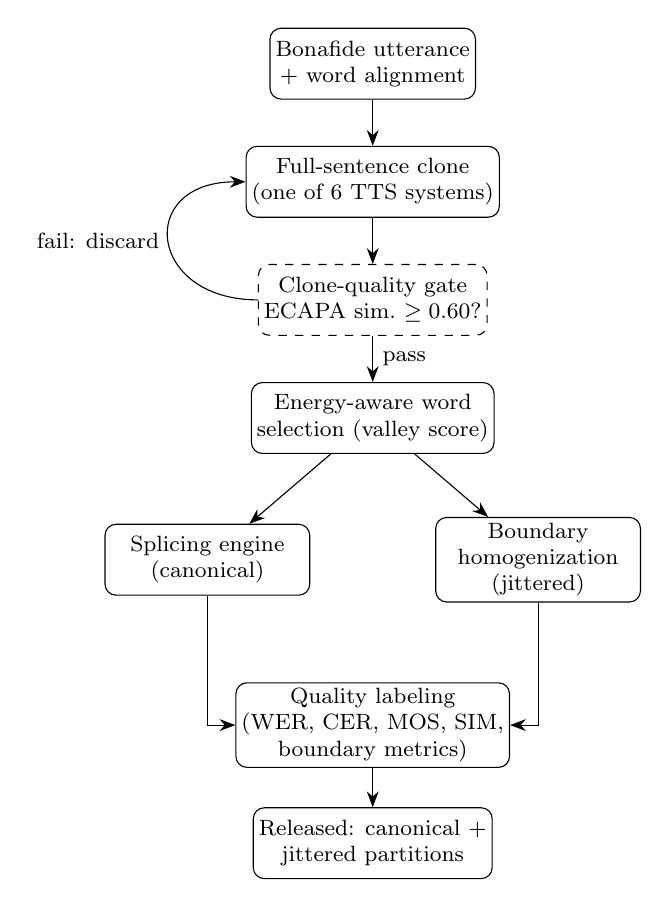
\begin{tikzpicture}[
  box/.style={draw, rounded corners, align=center, minimum width=2.6cm,
              minimum height=0.9cm, font=\footnotesize, inner sep=2pt},
  gate/.style={box, dashed},
  arr/.style={-{Stealth[length=2mm]}}
]
\node[box] (input) at (0,0) {Bonafide utterance\\+ word alignment};
\node[box] (clone) at (0,-1.5) {Full-sentence clone\\(one of 6 TTS systems)};
\node[gate] (gate) at (0,-3.0) {Clone-quality gate\\ECAPA sim.\ $\geq 0.60$?};
\node[box] (select) at (0,-4.5) {Energy-aware word\\selection (valley score)};
\node[box] (canon) at (-2.1,-6.3) {Splicing engine\\(canonical)};
\node[box] (jitter) at (2.1,-6.3) {Boundary\\homogenization\\(jittered)};
\node[box] (quality) at (0,-8.4) {Quality labeling\\(WER, CER, MOS, SIM,\\boundary metrics)};
\node[box] (output) at (0,-9.9) {Released: canonical +\\jittered partitions};

\draw[arr] (input) -- (clone);
\draw[arr] (clone) -- (gate);
\draw[arr] (gate) -- node[right,font=\footnotesize]{pass} (select);
\draw[arr] (gate.west) .. controls +(-1.4,0) and +(-1.4,0) ..
  node[left,font=\footnotesize]{fail: discard} (clone.west);
\draw[arr] (select) -- (canon);
\draw[arr] (select) -- (jitter);
\draw[arr] (canon.south) |- (quality.west);
\draw[arr] (jitter.south) |- (quality.east);
\draw[arr] (quality) -- (output);
\end{tikzpicture}
\caption{Partial-spoof pipeline overview. A failed clone-quality check
discards the clone as a generation failure rather than an attack
(Cloning and word extraction); the canonical and boundary-homogenized
(jittered) branches are released as separate sentence-disjoint
partitions but pass through the same quality-labeling stage.}
\label{fig:partialpipeline}
\end{figure}

\paragraph{Cloning and word extraction.} Rather than synthesizing each
replacement word in isolation (which yields flat, citation-form prosody
that is trivially detectable), the pipeline clones the \emph{full}
sentence in the target voice with one of the six previously described
TTS systems, and extracts the required words from the full synthesized
utterance by word-level alignment.
In-context words carry natural coarticulation and prosody, making the
splice harder to detect. Only utterances whose ECAPA-TDNN similarity to the
target speaker is at least 0.60 proceed to splicing. Below-threshold
clones do not resemble the target and are treated as generation
failures, not attacks. A consequence of this gate is that systems whose
clones sit well below 0.60 contribute little to the partial-spoof tier.
OpenVoice (mean similarity 0.388) is effectively absent from it,
contributing only 53 of the 18{,}421 partial-spoof samples, while the
higher-similarity systems dominate (OmniVoice alone accounts for
10{,}990). The tier's per-system composition is therefore narrower than
that of the full-spoof tier; the counts obtained are given in
Table~\ref{tab:pscomp}.

\paragraph{Energy-aware word selection.} Candidate replacement words are
not chosen at random. The goal is to place each splice seam where it is
least audible, e.g., within pauses rather than in the middle of connected speech.
To find such seams, every word boundary $b$ in the cloned audio is given
a \emph{valley score} $s(b)$. Let $W_b$ denote the set of short-time
analysis frames whose centers lie within $\pm 100$\,ms of the boundary,
let $N_b = |W_b|$ be the number of such frames, and let
$\mathrm{RMS}(t) \ge 0$ be the root-mean-square energy of frame $t$
(frames are 5\,ms long, thus $N_b = 40$ away from the signal edges). The
score is
\begin{equation}
s(b) \;=\; \frac{\displaystyle\min_{t \in W_b} \mathrm{RMS}(t)}
                 {\displaystyle\frac{1}{N_b}\sum_{t \in W_b} \mathrm{RMS}(t)}
\label{eq:valleyscore}
\end{equation}

That is, the quietest instant in the window divided by the window's
average loudness. Since RMS energy is non-negative and a minimum can
never exceed the corresponding mean, $s(b) \in [0,1]$ by construction. A
boundary that falls in clear inter-word silence has almost no energy at
its quietest instant, thus $s(b) \to 0$. A boundary buried in continuous
speech never quiets down within the window, thus $s(b) \to 1$. Only
words whose boundary score falls below a configurable threshold, and
whose duration exceeds a minimum, are eligible for replacement. Eligible
words are then selected greedily, lowest-$s(b)$ (quietest boundary)
first, subject to a non-adjacency constraint (selected word indices
differ by at least two). This distributes the spoofed content across
the utterance rather than forming a single contiguous block that would
resemble a segment-level rather than a word-level attack.

\paragraph{Splicing engine.} Figure~\ref{fig:splicesteps} shows the five
steps the engine applies to each replacement. First, it refines the
Parakeet word boundaries by local energy analysis, correcting the
100--\SI{300}{\milli\second} drift the transducer can exhibit on fast
connected speech. Second, it snaps each cut outward onto the nearest
silence, placing the seam in low energy. Third, it inserts the cloned
word at its \emph{natural} duration, with no time-stretching, preserving
the clone's pitch. Fourth, it matches the cloned word's loudness to a
voiced-RMS anchor computed once from the bonafide host, removing loudness
as a possible spoof cue. Fifth, it blends the seams with a
crossfade whose extent is bounded by the available silence on each side,
keeping the fade from bleeding a neighboring word into the splice. For
multi-word tiers, a running offset maps each subsequent cut onto the
current audio after earlier insertions have changed its length.

\begin{figure}[t]
\centering
\begin{tikzpicture}[
  node distance=4mm,
  step/.style={draw, rounded corners, align=center, minimum width=2.3cm,
               minimum height=1.6cm, font=\footnotesize},
  arr/.style={-{Stealth[length=2mm]}}
]
\node[step] (s1) {1.\ Refine\\word boundaries\\(energy analysis)};
\node[step, right=of s1] (s2) {2.\ Snap cuts\\to nearest\\silence};
\node[step, right=of s2] (s3) {3.\ Insert clone\\at natural\\duration};
\node[step, right=of s3] (s4) {4.\ Match\\loudness to\\voiced-RMS anchor};
\node[step, right=of s4] (s5) {5.\ Blend seams\\with bounded\\crossfade};
\draw[arr] (s1) -- (s2);
\draw[arr] (s2) -- (s3);
\draw[arr] (s3) -- (s4);
\draw[arr] (s4) -- (s5);
\end{tikzpicture}
\caption{The five-step splicing engine applied to each word replacement.
Steps 1--2 place the seam; step 3 preserves the clone's natural pitch by
avoiding time-stretching; step 4 removes loudness as a possible spoof
cue; step 5 smooths the seam within the available silence budget.}
\label{fig:splicesteps}
\end{figure}

The crossfade seam is drawn per splice from seven techniques in fixed
proportions (see Table~\ref{tab:splice}), ranging from a hard cut to several
equal-gain and equal-power fade laws. Randomizing the seam prevents a
detector from keying on a single fade signature. A single overlap
duration is drawn per splice from a fixed range and then bounded by the
available silence; there are no per-technique duration ranges.

\begin{table}[t]
\centering
\caption{Partial-spoof tier composition (18{,}421 spliced utterances),
by generating system, replacement tier, boundary-jitter partition, and
quality flag.}
\label{tab:pscomp}
\small
\begin{tabular}{lr@{\hskip 1.5em}lr}
\toprule
\textbf{System} & \textbf{Count} & \textbf{Breakdown} & \textbf{Count} \\
\midrule
OmniVoice   & 10{,}990 & W1 (1 word)       & 10{,}276 \\
Qwen3-TTS   &  1{,}565 & W2 (2 words)      &  5{,}991 \\
Chatterbox  &  3{,}423 & W3 (3 words)      &  2{,}154 \\
FishGram    &  1{,}317 & \emph{canonical}  &  8{,}456 \\
OuteTTS     &  1{,}073 & \emph{jittered}   &  9{,}965 \\
OpenVoice   &     53   & flag high/med/low & 4{,}875 / 13{,}072 / 474 \\
\midrule
\textbf{Total} & \textbf{18{,}421} & & \\
\bottomrule
\end{tabular}
\end{table}

\begin{table}[t]
\centering
\caption{Splice seam techniques and their sampling
proportions, as implemented. Fade-in curves are given for
$t\in[0,1]$; the fade-out is the time-reverse. Method~5 applies the
square-root (equal-power) law $\sqrt{t}$.}
\label{tab:splice}
\small
\begin{tabular}{clcc}
\toprule
\textbf{\#} & \textbf{Technique} & \textbf{Fade-in curve} & \textbf{Proportion} \\
\midrule
1 & Hard cut (no fade)          & ---                       & 10\% \\
2 & Overlap-add, Hann window    & $0.5(1-\cos\pi t)$        & 20\% \\
3 & Linear                      & $t$                       & 15\% \\
4 & Cosine (equal-power)        & $\sin(\pi t/2)$           & 20\% \\
5 & Square-root (equal-power)   & $\sqrt{t}$                & 15\% \\
6 & Logarithmic                 & $\log(1+9t)/\log 10$      & 10\% \\
7 & Inverted parabola           & $1-(1-t)^2$               & 10\% \\
\bottomrule
\end{tabular}
\end{table}

\paragraph{Boundary-homogenization variant.} Because a naive partial
spoof leaves only the two boundaries flanking the replaced word
anomalous, a detector can exploit the presence of a single discontinuous
boundary as a shortcut, achieving low error without learning any
synthesis artifact \citep{negroni2024splicing}. MARSA includes a
parallel \emph{jittered} variant of the partial-spoof tier that
suppresses this shortcut. In it, \emph{every} internal word boundary of
an utterance (genuine as well as spliced) independently undergoes, with
probability 0.5, one of three structural manipulations chosen uniformly
(distinct from the seven crossfade techniques of Table~\ref{tab:splice},
which shape the splice seam itself):
(i) A short truncation of one word's edge (10--\SI{40}{\milli\second}, kept
below the duration of a Spanish syllable nucleus to preserve
intelligibility). (ii) A Hann-windowed overlap of the two words
(30--\SI{80}{\milli\second}, matching the crossfade range used by prior
partial-spoof work \citep{luong2024llama}). (3) A bleed of one word's
edge into its neighbor (20--\SI{60}{\milli\second}, covering Spanish
voice-onset time plus a consonant-vowel transition). Setting the
manipulation probability to 0.5 maximizes the entropy of the
``manipulations per boundary'' signal, thus the spliced boundary is
no longer distinguishable by the mere fact of being manipulated. The jittered variant is released as a separate
sentence-disjoint partition, thus detectors can be trained and
evaluated on the canonical and homogenized distributions independently or
jointly.

\paragraph{Quality labeling without filtering.} The partial-spoof
generation pipeline computes WER, character-error rate, MOS, ECAPA similarity, and
boundary metrics for every sample, but does \emph{not} discard
low-quality samples. Each sample instead carries a categorical
\texttt{quality\_flag} (high/medium/low). Downstream users may stratify
or filter on it. Only structural failures (zero successfully spliced
words or missing or unreadable audio) are removed, since those are
not partial spoofs at all. This ``keep-everything, label-everything''
policy
reflects the fact that a real attacker does not post-filter output, and a
detector trained only on clean attacks may collapse on noisy ones.

% JCVASQUEZ UP TO HERE

\subsection*{Acoustic augmentation}

To support the study of channel robustness without regenerating
attacks, MARSA provides an augmentation layer that transforms the base
corpus into a channel-degraded training set. The layer is applied
identically to bonafide and spoof audio. Therefore, the augmentation type, the augmentation rate, and
the output loudness are all decoupled from the class label. In particular,
every file is loudness normalized by the same policy, thus neither the presence of an
augmentation nor its output level can serve as a shortcut cue for the
class. Without this discipline a detector can learn ``augmented implies
one class'' or ``louder implies one class'' and collapse at evaluation
time on clean, uniformly scaled audio.

\paragraph{Copies per file.} For each original training file the layer
emits one clean copy plus a number of augmented copies set by the 
corpus-multiplication factor. At the smallest factor
roughly one third of the training set stays clean; larger factors lower
that fraction. The development and evaluation splits are released at
factor one and are never augmented, thus model selection and testing
occur on clean audio.

\paragraph{Augmentation mode.} Per augmented clip, a probability gate
selects the mode. With probability 0.6 a single family is applied,
choosing between reverberation-plus-noise and codec degradation in a
60:40 ratio; with probability 0.4 the two are \emph{stacked},
reverberation and noise first and then a codec round-trip on the result,
which models the common real-world case of a reverberant, noisy source
transmitted over a lossy channel. The augmentation chain is recorded in
the sample's system identifier, with a pipe separator for stacked clips
(for example \texttt{RIR\_SMALL\_NOI\_SNR15|CODEC\_OPUS\_LOSS3PCT}),
keeping the full history recoverable from the protocol file and
requiring no directory restructuring. The layer is released at four
corpus-multiplication factors ($\times$2, $\times$3, $\times$5,
$\times$10). The same factor is applied to bonafide and spoof alike. The
clean fraction is therefore identical across classes, and augmentation
does not shift the class balance. Rebalancing the (naturally spoof-heavy) corpus
is deliberately left to the user at training time rather than baked into
the data (see Usage Notes), which keeps augmentation from becoming a
class cue.

\paragraph{Reverberation and noise.} This family convolves the clip with
a room impulse response drawn from the RIRS\_NOISES set \citep{ko2017rir},
stratified into small, medium, and large rooms (sampled at 30\%, 50\%,
and 20\%), then mixes additive noise drawn from MUSAN \citep{musan}. The
noise source is ambient noise, multi-speaker babble, or music (sampled
at 50\%, 30\%, and 20\%), and it is mixed at a signal-to-noise ratio
sampled from three bands, 0--5\,dB, 5--30\,dB, and 30--35\,dB, weighted
10\%, 80\%, and 10\%. Most clips therefore sit in a moderate-degradation
regime with a light tail at each extreme.

\paragraph{Codec degradation.} This family applies a real
encode-then-decode round-trip through six telephony and VoIP codecs,
covering the channels most representative of the target deployment:
G.711 mu-law and A-law (PSTN and landline), AMR-NB (2G/3G mobile), Speex
(legacy VoIP), Opus (the dominant over-the-top codec, used by consumer
messaging and conferencing apps), and AAC (broadband). Speex substitutes
for iLBC in this slot, because iLBC proved unobtainable in any ffmpeg
build we tested, static or system, whereas AMR-NB and AAC required a pinned
static ffmpeg build (Code Availability) rather than a stock system
installation. For codecs with a selectable bitrate a bitrate is drawn
from the encoder's supported set, and with a fixed probability an
additional packet-loss simulation is applied at a sampled loss fraction.
The signal is resampled to each codec's native rate for the round-trip
and back to \SI{16}{\kilo\hertz} on write. All six codecs are realized
in the released corpus, each within 0.2 percentage points of its target
mix weight (Technical Validation). This configured codec set was chosen
for deployment realism; a broader design that adds wideband and
enterprise codecs together with a burst-loss channel model and per-codec
packet-loss concealment is documented as a planned extension but is not
part of the released corpus.

\paragraph{Training-time augmentation.} A convolutive and additive
signal-level augmentation of the RawBoost family \citep{tak2022ssl} is
intended to be applied on the fly during detector training rather than
baked into the released corpus. It is a fast, waveform-level operation with no benefit to
pre-computation. It is therefore documented here and provided in the
accompanying code, but is not part of the deposited files.

\subsection*{Parameter summary}

Table~\ref{tab:params} lists the numeric parameters that govern
generation; the corpus can be regenerated from the released code
together with these values. All stochastic choices are driven by a
fixed base seed (42) combined with a per-sample key hash, making the
assignment of attack systems, word selections, splice techniques, and
jitter plans deterministic and reproducible across runs.

\begin{table}[t]
\centering
\caption{Key generation parameters. Distributions are written as
value~(probability); intervals sampled uniformly are written
Uniform$[a,b]$.}
\label{tab:params}
\small
\begin{tabular}{p{4.9cm}p{6.6cm}}
\toprule
\textbf{Parameter} & \textbf{Value} \\
\midrule
\multicolumn{2}{l}{\emph{Full-spoof screening}} \\
\midrule
WER rejection ceiling & 0.15 (hard gate) \\
CER rejection ceiling & 0.10 (hard gate) \\
NISQA MOS, speaker similarity & recorded, not used as a rejection gate \\
Regeneration budget & up to 5 rounds on structural failure \\
\midrule
\multicolumn{2}{l}{\emph{Partial-spoof: word selection}} \\
\midrule
Tier minimum sentence length & W1: 4, W2: 8, W3: 12 words \\
Non-adjacency constraint & selected word indices differ by $\geq 2$ \\
Valley-score window / frame & $\pm$\SI{100}{\milli\second} / \SI{5}{\milli\second} \\
Valley-score eligibility & combined score $\leq 0.65$ \\
Minimum word duration & \SI{200}{\milli\second} \\
Clone acceptance gate & ECAPA-TDNN cosine similarity $\geq 0.60$ \\
\midrule
\multicolumn{2}{l}{\emph{Partial-spoof: splice engine}} \\
\midrule
Energy-refinement radius & \SI{300}{\milli\second} \\
Silence RMS threshold & 0.015 (of full scale) \\
Valley-snap search half-width & \SI{50}{\milli\second} \\
Crossfade overlap & Uniform$[30,80]$~ms, clamped to the inter-word gap \\
Splice-technique proportions & see Table~\ref{tab:splice} \\
Loudness match & per-utterance voiced-RMS anchor; frame \SI{20}{\milli\second}; voiced gate $0.15\times$P95; peak ceiling 0.99 \\
\midrule
\multicolumn{2}{l}{\emph{Boundary-jitter variant}} \\
\midrule
Per-boundary manipulation prob. & 0.50 \\
Truncate / overlap / bleed range & Uniform$[10,40]$ / $[30,80]$ / $[20,60]$~ms \\
\midrule
\multicolumn{2}{l}{\emph{Augmentation}} \\
\midrule
Family mix & RIR+noise 0.60, codec 0.40 \\
Stacking-gate probability & 0.40 (RIR+noise then codec) \\
Room size & small 0.30, medium 0.50, large 0.20 \\
Noise source & noise 0.50, babble 0.30, music 0.20 \\
SNR band (dB) & $[0,5]$ (0.10), $[5,30]$ (0.80), $[30,35]$ (0.10) \\
Codec weights & G.711$\mu$ 0.25, G.711A 0.15, AMR-NB 0.20, iLBC 0.05, Opus 0.25, AAC 0.10 \\
Codec bitrates (kbps) & AMR-NB $\{4.75\text{--}12.2\}$; Opus $\{8,12,16,24,32\}$; AAC $\{24,32,48,64\}$; G.711/iLBC fixed \\
Packet loss & applied with prob.\ 0.30; fraction Uniform$[0,0.05]$ \\
Multiplication factors & $\times$2, $\times$3, $\times$5, $\times$10; same factor applied to both classes \\
\midrule
\multicolumn{2}{l}{\emph{Quality-flag thresholds (partial spoof)}} \\
\midrule
high & WER $\leq 0.10$ and NISQA MOS $\geq 4.0$ and SIM $\geq 0.50$ \\
medium & WER $\leq 0.30$ (and not high) \\
low & otherwise \\
\bottomrule
\end{tabular}
\end{table}

% =====================================================================
\section*{Data Records}

\PENDING{Zenodo deposit DOI and record URL.} The corpus is deposited in
the Zenodo open repository under a single versioned record.

The release is organized to mirror the ASVspoof2019 Logical Access (LA)
convention, which anti-spoofing training and evaluation code already
understands. Each tier is provided as a flat directory of FLAC audio
files accompanied by a protocol text file. Each protocol line names the
speaker, the utterance identifier, the system identifier, and the
class label:

\begin{quote}\small
\texttt{arf\_00295\ LA\_T\_12000000\ FISHGRAM\_PSW1\ partial\_spoof}
\end{quote}

Class labels are \texttt{bonafide}, \texttt{spoof} (full synthesis), and
\texttt{partial\_spoof}. System identifiers encode the generating system
and, for partial spoof, the tier: \texttt{PSW1}/\texttt{PSW2}/%
\texttt{PSW3} for one/two/three replaced words, with a trailing
\texttt{J} for the boundary-homogenized (jittered) variant. Utterance
identifiers are assigned in disjoint numeric ranges per tier and
variant; they never collide across the corpus. For the
partial-spoof tier, a companion table lists, for every spoofed word, its
start and end time within the released (spliced) audio and the splice
technique used; these constitute the frame-level spoof labels. Per-sample
metadata (the acoustic-quality metrics and \texttt{quality\_flag}
described in Methods) are provided as CSV tables aggregated across all
pipelines.

The composition of the partial-spoof tier is given in
Table~\ref{tab:pscomp}. It reflects the corpus-construction weighting
(OmniVoice is the majority attack) and the effect of the ECAPA clone
gate (OpenVoice is nearly excluded), and it is dominated by the W1 tier
because most eligible utterances are short enough to admit only a
single replacement. All 18{,}421 samples are released, unfiltered by
quality; the recommended clean partition is identifiable directly from
the released per-sample metrics (Technical Validation; see also Usage
Notes).

The augmentation tiers reuse the same protocol convention, with the
augmentation chain recorded in the system identifier field as described
above.

\PENDING{Final on-disk size of the deposited record, and the exact
top-level directory tree, to be inserted once the deposit is finalized.}

% =====================================================================
\section*{Technical Validation}

Two forms of evidence establish that MARSA is fit for its purpose:
intrinsic quality of the generated audio, and extrinsic usefulness for
training an anti-spoofing detector.

\subsection*{Intrinsic quality of generated attacks}

Every generated utterance was screened for intelligibility, perceptual
quality, and speaker fidelity, using three metrics computed during
generation (Methods). Word-error rate (WER) is measured against the
target text from a Parakeet re-transcription of the generated audio.
Perceptual quality is the mean opinion score (MOS) predicted by the
NISQA no-reference speech-quality model \citep{nisqa}; NISQA outputs
five quality dimensions (overall MOS, noisiness, discontinuity,
coloration, and loudness), of which only the overall MOS is used here.
Speaker fidelity is ECAPA-TDNN speaker-embedding cosine similarity to
the target speaker \citep{ecapa}, the same embedding model and
similarity measure used to deduplicate speakers between HABLA and Common
Voice in the bonafide source corpus (Methods), where speakers exceeding
0.75 cosine similarity to an existing HABLA speaker were excluded.
Per-system yields and mean values for the full-spoof screening metrics
are reported in Table~\ref{tab:fullspoof}.

\begin{table}[t]
\centering
\caption{Full-spoof pipelines: post-screening utterance yields and mean
acoustic-quality metrics. WER is word-error rate against the target
text; MOS is the overall mean opinion score predicted by the NISQA
no-reference speech-quality model \citep{nisqa} (1--5, higher better;
NISQA also predicts four other quality dimensions, not used here); SIM
is ECAPA-TDNN cosine speaker similarity to the target (higher better).}
\label{tab:fullspoof}
\small
\begin{tabular}{lrccc}
\toprule
\textbf{System} & \textbf{Utterances} & \textbf{WER (\%)} & \textbf{MOS} & \textbf{SIM} \\
\midrule
Fish-Speech (FishGram) & 34{,}197 & 2.17 & 4.57 & 0.602 \\
Qwen3-TTS              & 31{,}568 & 1.46 & 4.37 & 0.720 \\
OpenVoice v2           & 29{,}796 & 1.50 & 4.38 & 0.388 \\
Chatterbox             & 31{,}701 & 1.20 & 4.39 & 0.714 \\
OuteTTS                & 25{,}642 & 2.36 & 4.45 & 0.462 \\
OmniVoice              & 33{,}743 & 1.06 & 4.28 & 0.686 \\
\midrule
\textbf{Total}         & \textbf{186{,}647} & & & \\
\bottomrule
\end{tabular}
\end{table}

The systems differ deliberately in cloning fidelity. Speaker similarity
spans a wide band, from 0.388 (OpenVoice, whose tone-conversion
architecture lets the synthesis base voice bleed through) through 0.462
(OuteTTS) and the high-fidelity cluster of Qwen3-TTS (0.720), Chatterbox
(0.714), and OmniVoice (0.686); perceptual quality (NISQA MOS) is
uniformly high, from 4.28 to 4.57, and WER against the target text is at or below
2.4\% for every system. This spread is deliberate. A detector trained on
MARSA sees both high-fidelity and low-fidelity attacks rather than a
single narrow band of synthesis quality, and these figures confirm that
the attacks are intelligible, natural-sounding, and (for the stronger
systems) close to the target speaker, that is, credible spoofing
attempts rather than degenerate synthesis. For the partial-spoof tier, quality metrics
are computed per sample and released as labels rather than used as
filters. The corpus therefore spans the full realistic quality range;
under the resulting \texttt{quality\_flag} the 18{,}421 spliced samples
divide into 4{,}875 high, 13{,}072 medium, and 474 low, and 15{,}641
(84.9\%) pass the full-spoof intelligibility gate (WER $\leq 0.15$,
CER $\leq 0.10$) that defines the recommended clean partition.
Table~\ref{tab:pstierquality} reports WER, CER, NISQA, and speaker
similarity broken down by replacement tier, computed over the released
per-sample metrics.

\begin{table}[t]
\centering
\caption{Partial-spoof quality by replacement tier, computed from the
released per-sample metrics. WER and CER are against the target
transcript; NISQA is the no-reference perceptual-quality score; SIM is
ECAPA-TDNN cosine similarity between the spliced result and the target
speaker, naturally higher than full-spoof SIM (Table~\ref{tab:fullspoof})
since most of a partial-spoof utterance is genuine audio. The splice
engine does not record a boundary-drift measurement directly; the
closest released quantity is the effective crossfade duration applied at
each seam, reported here instead.}
\label{tab:pstierquality}
\small
\begin{tabular}{lrccccc}
\toprule
\textbf{Tier} & \textbf{Utt.} & \textbf{WER (\%)} & \textbf{CER (\%)} & \textbf{NISQA} & \textbf{SIM} & \textbf{Crossfade (ms)} \\
\midrule
W1 (1 word)  & 10{,}276 & 4.61 & 2.36 & 3.53 & 0.781 & 4.87 \\
W2 (2 words) &  5{,}991 & 6.08 & 3.25 & 3.28 & 0.799 & 4.31 \\
W3 (3 words) &  2{,}154 & 6.80 & 3.74 & 3.14 & 0.820 & 3.89 \\
\midrule
\textbf{Total} & \textbf{18{,}421} & 5.34 & 2.81 & 3.40 & 0.791 & 4.41 \\
\bottomrule
\end{tabular}
\end{table}

\subsection*{Bonafide transcription reliability}

Parakeet TDT is used for two distinct purposes in the pipeline, and only
one of them concerns the bonafide utterances directly. First, every
individual bonafide utterance is transcribed once (Bonafide source
corpus); this per-utterance transcript is not used by full-spoof at all,
but it is load-bearing for partial-spoof, where it supplies both the
text handed to the cloning system and the word-level timestamps used for
splice alignment, because partial-spoof requires timing information tied
to the exact bonafide recording being edited, which no external
transcript can supply (Partial-spoof pipeline). Second, Parakeet is run
again, separately, on each speaker's \emph{concatenated reference clip}
(a different audio object, built by joining several bonafide files
together), purely to give the full-spoof systems that use one a text
hint describing what that reference clip says. The content a full-spoof
system is actually asked to synthesize is independent of both of these
transcription steps. It is drawn directly from the original Common Voice
sentence, not from any ASR output (Full-spoof attack pipelines).

We validated the accuracy of the first of these, the per-utterance
transcription stage that partial-spoof depends on, against an
independent ground truth. For the Common-Voice-origin bonafide subset,
where Common Voice's own original sentence serves as that ground truth,
we compared it to Parakeet's transcript of the same audio.
Table~\ref{tab:parakeetwer} reports word error rate (WER) and character
error rate (CER) overall and per accent. Overall WER is 3.02\% and CER
is 0.87\%, consistent with Parakeet TDT's published Spanish performance
\citep{parakeet}. These figures indicate that the word-level timestamps
underlying the partial-spoof tier are anchored to a transcription stage
with error rates in line with expectations for the ASR model, rather
than to unvalidated output.

\begin{table}[t]
\centering
\caption{Parakeet TDT transcription accuracy against original Common
Voice ground-truth sentences, for the Common-Voice-origin bonafide
subset (12{,}415 of 13{,}111 selected utterances matched a cached
transcript; 696 fell below the four-word transcription minimum,
Methods). Venezuelan is shown for completeness but excluded from the
Overall row and from per-accent conclusions, since only one Venezuelan
speaker passed the Common Voice speaker-similarity filter (Bonafide
source corpus), leaving $n=4$, too few for a reliable estimate.}
\label{tab:parakeetwer}
\small
\begin{tabular}{lrcc}
\toprule
\textbf{Accent} & \textbf{n} & \textbf{WER (\%)} & \textbf{CER (\%)} \\
\midrule
Chilean       &  1{,}247 & 1.93 & 0.48 \\
Peninsular    &  5{,}109 & 2.54 & 0.66 \\
Colombian     &    791 & 3.02 & 0.84 \\
Mexican       &  5{,}264 & 3.74 & 1.18 \\
Venezuelan ($n{=}4$) &   4 & 8.33 & 1.61 \\
\midrule
\textbf{Overall} & \textbf{12{,}415} & \textbf{3.02} & \textbf{0.87} \\
\bottomrule
\end{tabular}
\end{table}

\subsection*{Augmentation fidelity}

The augmentation layer's realized codec mix was verified against its
configured target weights (Parameter summary) on the released corpus:
every one of the six codecs occurs within 0.2 percentage points of its
target proportion. AMR-NB and Speex, the two narrowband codecs in the
mix, were additionally confirmed spectrally to carry no energy above
\SI{4}{\kilo\hertz}, consistent with their native encoding bandwidth and
confirming that the codec round-trip degrades the signal as intended
rather than passing it through unaltered.

\subsection*{Baseline anti-spoofing detection}

\PENDING{Baseline detector results. A standard open anti-spoofing
countermeasure (for example RawNet2 \citep{rawnet2} or AASIST
\citep{aasist}) is to be trained and evaluated on MARSA, reporting
equal-error rate (EER) overall and broken down by (i) attack system,
(ii) partial-spoof tier, (iii) accent group, and (iv) augmentation
condition, together with a cross-condition matrix (train on one
condition, test on another) to demonstrate the corpus's value for
studying generalization. This experiment has not yet been run and is the
final prerequisite for submission. The baseline model choice is not yet
fixed.}

The intended baseline protocol is a speaker-disjoint train/development/
evaluation split, EER as the primary metric, and a cross-condition
generalization matrix that quantifies how much detection degrades when
the test attack system, dialect, or channel condition is unseen during
training. Because MARSA controls the splice-boundary shortcut through its
jittered variant, the protocol also includes training on the canonical
partial-spoof partition and testing on the jittered partition (and vice
versa), which isolates whether a detector has learned the boundary
anomaly or the underlying synthesis artifact.

% =====================================================================
\section*{Usage Notes}

\paragraph{Recommended splits and balancing.} MARSA preserves the source
corpus's speaker and accent imbalance (Table~\ref{tab:accents}). Users
training detectors should adopt a speaker-disjoint split to avoid
speaker leakage, and should apply class and accent balancing at training
time (for example via weighted sampling or a class-weighted loss) rather
than expecting the corpus to be pre-balanced. Augmentation deliberately
does not rebalance the classes. The same multiplication factor is
applied to both bonafide and spoof, and every tier therefore preserves
the source class ratio; augmentation cannot leak the class label
through a differing clean fraction.

\paragraph{Recommended clean partial-spoof subset.} The full partial-spoof
tier (18{,}421 samples) is released unfiltered, retaining the noisier
tail for studies that need it. For most training use we recommend the
subset that passes the same intelligibility gate applied to the
full-spoof tier, WER $\leq 0.15$ and CER $\leq 0.10$. This retains
15{,}641 samples (84.9\%) and can be selected directly from the released
per-sample \texttt{wer} and \texttt{cer} columns. Using it also makes the
intelligibility criterion consistent across the full-spoof and
partial-spoof tiers. The filter is close to uniform across systems
(each loses 9--18\%) and therefore does not distort the tier's system
composition.

\paragraph{Frame-level vs utterance-level use.} The partial-spoof tier
supports both utterance-level detection (is any part of this signal
spoofed?) and localization (which frames are spoofed?), the latter via
the released per-word boundary table. Note that these boundaries index
the released spliced audio, not the original bonafide recording, because
the spliced audio's total duration differs from the source.

\paragraph{The jittered partition.} Researchers studying detector
shortcuts should train and evaluate on the canonical and jittered
partial-spoof partitions separately; a detector that performs well on the
canonical partition but poorly on the jittered one has likely learned the
boundary-anomaly shortcut rather than a synthesis-artifact feature.

\paragraph{Augmentation.} The four augmentation factors are supersets of
one another in construction intent but are released as independent tiers;
users should select a single factor appropriate to their compute budget
rather than pooling all four, which would over-represent augmented
variants of the same source utterances.

\paragraph{Ethical use.} MARSA is released to support the development of
\emph{defensive} anti-spoofing systems. The synthetic audio it contains
is generated from open TTS systems applied to a consenting-speaker
research corpus. It must not be used to impersonate real individuals.
Note that the released audio is deliberately \emph{not} watermarked (see
Methods). The two systems that watermark by default were reverted to
watermark-free generation, making the corpus test synthesis-artifact
detection rather than watermark detection. \PENDING{Confirm the licensing
terms of each constituent TTS system permit redistribution of generated
audio, and state the corpus license.}

% =====================================================================
\section*{Code Availability}

\PENDING{Public code repository URL.} The full generation pipeline (the
six full-spoof attack systems' wrappers, the partial-spoof splicing
engine, the boundary-homogenization variant, and the augmentation
layer) is released as open-source software, with the exact configuration
and random seeds used to produce the released corpus. The pipeline is
implemented in Python and orchestrated to make each tier reproducible
from the bonafide source. The codec-degradation family (Acoustic
augmentation) requires a static ffmpeg build with AMR-NB and AAC
encoding support (a stock system ffmpeg typically lacks both); the
pinned build used to generate the released corpus is included with the
repository rather than assumed to be present on the host system.

\section*{Data Availability}

\PENDING{Zenodo record DOI.} All MARSA audio, protocol files, frame-level
label tables, and per-sample metadata are openly available from the
Zenodo repository under the record cited above. The bonafide source
recordings derive from HABLA \citep{habla}; users requiring the original
unprocessed bonafide audio should additionally consult that resource.

% =====================================================================
\section*{Acknowledgements}
\PENDING{Funding sources, compute provider, and advisor acknowledgement.}

\section*{Author Contributions}
\PENDING{Per-author contribution statement (CRediT taxonomy).}

\section*{Ethics Declaration}
The bonafide recordings originate from the HABLA corpus of
consenting-speaker Spanish speech \citep{habla}, and MARSA introduces no
new human-subjects data collection beyond that source. \PENDING{State the
consent and ethics basis of the upstream bonafide corpus, its
redistribution license, and confirm the derivative-redistribution chain
end to end.} The synthetic tiers are produced by applying open
text-to-speech systems to this corpus for the express purpose of
\emph{defensive} anti-spoofing research. To keep that purpose intact,
the released audio is watermark-free by design (see Methods). The two
systems that watermark by default were reverted to watermark-free
generation, forcing detectors to learn synthesis artifacts rather than
watermarks. This is a dual-use resource; it must not be used to
impersonate real individuals or to build systems whose purpose is
deception, and it is released to strengthen detection, not evasion.

\section*{Competing Interests}
The authors declare no competing interests.

% =====================================================================
% Embedded bibliography (self-contained; no external .bib needed).
% =====================================================================
\begin{thebibliography}{99}

\bibitem{asvspoof2019}
M.~Todisco \emph{et al.},
``ASVspoof 2019: Future horizons in spoofed and fake audio detection,''
in \emph{Proc. Interspeech}, 2019, pp.~1008--1012.

\bibitem{asvspoof2021}
J.~Yamagishi \emph{et al.},
``ASVspoof 2021: Accelerating progress in spoofed and deepfake speech
detection,'' in \emph{Proc. ASVspoof 2021 Workshop}, 2021.

\bibitem{asvspoof5}
X.~Wang \emph{et al.},
``ASVspoof 5: Crowdsourced speech data, deepfakes, and adversarial
attacks at scale,'' in \emph{Proc. ASVspoof Workshop}, 2024.
\emph{arXiv:2408.08739}.

\bibitem{rawnet2}
H.~Tak \emph{et al.},
``End-to-end anti-spoofing with RawNet2,''
in \emph{Proc. ICASSP}, 2021.

\bibitem{tak2022ssl}
H.~Tak \emph{et al.},
``Automatic speaker verification spoofing and deepfake detection using
wav2vec 2.0 and data augmentation,''
in \emph{Proc. Odyssey}, 2022, pp.~112--119.

\bibitem{aasist}
J.-w.~Jung \emph{et al.},
``AASIST: Audio anti-spoofing using integrated spectro-temporal graph
attention networks,'' in \emph{Proc. ICASSP}, 2022.

\bibitem{sasvevalplan2022}
J.-w.~Jung \emph{et al.},
``SASV challenge 2022: A spoofing aware speaker verification challenge
evaluation plan,'' \emph{arXiv:2201.10283}, 2022.

\bibitem{sasv2022}
J.-w.~Jung \emph{et al.},
``SASV 2022: The first spoofing-aware speaker verification challenge,''
in \emph{Proc. Interspeech}, 2022. \emph{arXiv:2203.14732}.

\bibitem{raptor2026}
A.~Kulkarni, S.~Dowerah, A.~Kulkarni, T.~Alum\"{a}e, and M.~Magimai~Doss,
``Do compact SSL backbones matter for audio deepfake detection? A
controlled study with RAPTOR,'' in \emph{Proc. Interspeech}, 2026.
\emph{arXiv:2603.06164}.

\bibitem{dowerah2025speechdfarena}
S.~Dowerah \emph{et al.},
``Speech DF Arena: A leaderboard for speech deepfake detection models,''
\emph{arXiv:2509.02859}, 2025.

\bibitem{muller2026erodingtrust}
N.~M.~M\"uller and W.~H.~Choong,
``Eroding trust in real speech: A large-scale study of human audio
deepfake perception,'' \emph{arXiv:2605.26136}, 2026.

\bibitem{muller2022generalize}
N.~M.~M\"uller \emph{et al.},
``Does audio deepfake detection generalize?''
in \emph{Proc. Interspeech}, 2022, pp.~2783--2787.

\bibitem{muller2024harder}
N.~M.~M\"uller \emph{et al.},
``Harder or different? Understanding generalization of audio deepfake
detection,'' in \emph{Proc. Interspeech}, 2024.

\bibitem{habla}
P.~A.~Tamayo-Fl\'orez, R.~Manrique, and B.~Pereira Nunes,
``HABLA: A dataset of Latin American Spanish accents for voice
anti-spoofing,'' in \emph{Proc. Interspeech}, 2023, pp.~1963--1967.

\bibitem{commonvoice}
R.~Ardila \emph{et al.},
``Common Voice: A massively-multilingual speech corpus,''
in \emph{Proc. 12th Language Resources and Evaluation Conf. (LREC)},
2020, pp.~4218--4222.

\bibitem{forbes2019ceofraud}
J.~Damiani,
``A voice deepfake was used to scam a CEO out of \$243,000,''
\emph{Forbes}, Sep. 2019.
\url{https://www.forbes.com/sites/jessedamiani/2019/09/03/a-voice-deepfake-was-used-to-scam-a-ceo-out-of-243000/}

\bibitem{europol2022deepfakes}
Europol Innovation Lab,
``Facing reality? Law enforcement and the challenge of deepfakes,''
Europol, 2022.
\url{https://www.europol.europa.eu/cms/sites/default/files/documents/Europol_Innovation_Lab_Facing_Reality_Law_Enforcement_And_The_Challenge_Of_Deepfakes.pdf}

\bibitem{destefano2023testimony}
J.~DeStefano,
``Written testimony,''
U.S. Senate Judiciary Committee, Subcommittee on Human Rights and the
Law, Jun. 2023.
\url{https://www.judiciary.senate.gov/imo/media/doc/2023-06-13\%20PM\%20-\%20Testimony\%20-\%20DeStefano.pdf}

\bibitem{infobae2026whatsapp}
Infobae,
``\,`Mam\'a, necesito ayuda': la nueva estafa con IA que clona la voz de
tus hijos con solo 3 segundos de audio,''
Mar. 2026.
\url{https://www.infobae.com/tecno/2026/03/26/mama-necesito-ayuda-la-nueva-estafa-con-ia-que-clona-la-voz-de-tus-hijos-con-solo-3-segundos-de-audio/}

\bibitem{infobae2025colombia}
Infobae,
``Incrementan las estafas con voces clonadas con inteligencia
artificial en diciembre: cinco claves para detectarlas,''
Dec. 2025.
\url{https://www.infobae.com/colombia/2025/12/03/incrementan-las-estafas-con-voces-clonadas-con-inteligencia-artificial-en-diciembre-cinco-claves-para-detectarlas/}

\bibitem{yi2021had}
J.~Yi \emph{et al.},
``Half-truth: A partially fake audio detection dataset,''
in \emph{Proc. Interspeech}, 2021, pp.~1654--1658.

\bibitem{add2022}
J.~Yi \emph{et al.},
``ADD 2022: The first audio deep synthesis detection challenge,''
in \emph{Proc. ICASSP}, 2022. \emph{arXiv:2202.08433}.

\bibitem{kantharuban2023dialectgap}
A.~Kantharuban, I.~Vuli\'c, and A.~Korhonen,
``Quantifying the dialect gap and its correlates across languages,''
in \emph{Findings of EMNLP}, 2023.

\bibitem{nacimiento2024biases}
E.~Nacimiento-Garc\'ia, H.~S.~D\'iaz-Kaas-Nielsen, and
C.~S.~Gonz\'alez-Gonz\'alez,
``Gender and accent biases in AI-based tools for Spanish,''
\emph{Applied Sciences}, vol.~14, no.~11, p.~4734, 2024.

\bibitem{zuluaga2023commonaccent}
J.~Zuluaga-Gomez, S.~Ahmed, D.~Visockas, and C.~Subakan,
``CommonAccent: Exploring large acoustic pretrained models for accent
classification based on Common Voice,''
in \emph{Proc. Interspeech}, 2023, pp.~5291--5295.

\bibitem{zhang2023partialspoof}
L.~Zhang, X.~Wang, E.~Cooper, N.~Evans, and J.~Yamagishi,
``The PartialSpoof database and countermeasures for the detection of
short fake speech segments embedded in an utterance,''
\emph{IEEE/ACM Trans. Audio, Speech, Lang. Process.}, vol.~31,
pp.~813--825, 2023.

\bibitem{li2025hqmpsd}
M.~Li \emph{et al.},
``HQ-MPSD: A multilingual artifact-controlled benchmark for partial
deepfake speech detection,'' \emph{arXiv:2512.13012}, 2025.

\bibitem{hispaspoof}
M.~Risques, K.~Bhagtani, A.~K.~S.~Yadav, and E.~J.~Delp,
``HISPASpoof: A new dataset for Spanish speech forensics,''
in \emph{Proc. ICASSP}, 2026. \emph{arXiv:2509.09155}.

\bibitem{mlaad}
N.~M.~M\"uller \emph{et al.},
``MLAAD: The multi-language audio anti-spoofing dataset,''
in \emph{Proc. IJCNN}, 2024. \emph{arXiv:2401.09512}.

\bibitem{speechfake}
W.~Huang, Y.~Gu, Z.~Wang, H.~Zhu, and Y.~Qian,
``SpeechFake: A large-scale multilingual speech deepfake dataset
incorporating cutting-edge generation methods,''
in \emph{Proc. ACL}, 2025. \emph{arXiv:2507.21463}.

\bibitem{negroni2024splicing}
V.~Negroni, D.~Salvi, P.~Bestagini, and S.~Tubaro,
``Analyzing the impact of splicing artifacts in partially fake speech
signals,'' in \emph{Proc. ASVspoof 5 Workshop}, 2024.

\bibitem{huang2024detectable}
S.-F.~Huang \emph{et al.},
``Detecting the undetectable: Assessing the efficacy of current spoof
detection methods against seamless speech edits,''
in \emph{Proc. IEEE SLT}, 2024.

\bibitem{luong2024llama}
H.-T.~Luong, H.~Li, L.~Zhang, K.~A.~Lee, and E.~S.~Chng,
``LlamaPartialSpoof: An LLM-driven fake speech dataset simulating
disinformation generation,'' in \emph{Proc. ICASSP}, 2025.

\bibitem{fishspeech}
S.~Liao \emph{et al.},
``Fish-Speech: Leveraging large language models for advanced
multilingual text-to-speech synthesis,'' \emph{arXiv:2411.01156}, 2024.

\bibitem{qwen3tts}
Qwen Team, Alibaba Group,
``Qwen3-TTS technical report,'' \emph{arXiv:2601.15621}, 2026.

\bibitem{openvoice}
Z.~Qin, W.~Zhao, X.~Yu, and X.~Sun,
``OpenVoice: Versatile instant voice cloning,''
\emph{arXiv:2312.01479}, 2024.

\bibitem{chatterbox}
Resemble AI,
``Chatterbox: Open-source text-to-speech with neural watermarking,''
software release, 2025.
\url{https://github.com/resemble-ai/chatterbox}

\bibitem{outetts}
OuteAI,
``OuteTTS: LLM-based text-to-speech via discrete audio tokens,''
software release, 2025. \url{https://huggingface.co/OuteAI}

\bibitem{omnivoice}
H.~Zhu \emph{et al.},
``OmniVoice: Towards omnilingual zero-shot text-to-speech with diffusion
language models,'' \emph{arXiv:2604.00688}, 2026.

\bibitem{cosyvoice}
Z.~Du \emph{et al.},
``CosyVoice 3: Towards in-the-wild speech generation via scaling-up and
post-training,'' \emph{arXiv:2505.17589}, 2025.

\bibitem{ecapa}
B.~Desplanques, J.~Thienpondt, and K.~Demuynck,
``ECAPA-TDNN: Emphasized channel attention, propagation and aggregation
in TDNN based speaker verification,''
in \emph{Proc. Interspeech}, 2020, pp.~3830--3834.

\bibitem{nisqa}
G.~Mittag, B.~Naderi, A.~Chehadi, and S.~M\"oller,
``NISQA: A deep CNN-self-attention model for multidimensional speech
quality prediction with crowdsourced datasets,''
in \emph{Proc. Interspeech}, 2021, pp.~2127--2131.

\bibitem{tdt}
H.~Xu, F.~Jia, S.~Majumdar, S.~Watanabe, and B.~Ginsburg,
``Efficient sequence transduction by jointly predicting tokens and
durations,'' in \emph{Proc. ICML}, 2023.

\bibitem{parakeet}
NVIDIA NeMo Team,
``Parakeet-TDT-0.6B-v3: Multilingual token-and-duration transducer ASR,''
model release, 2024.
\url{https://huggingface.co/nvidia/parakeet-tdt-0.6b-v3}

\bibitem{mfa}
M.~McAuliffe, M.~Socolof, S.~Mihuc, M.~Wagner, and M.~Sonderegger,
``Montreal Forced Aligner: Trainable text-speech alignment using Kaldi,''
in \emph{Proc. Interspeech}, 2017, pp.~498--502.

\bibitem{musan}
D.~Snyder, G.~Chen, and D.~Povey,
``MUSAN: A music, speech, and noise corpus,''
\emph{arXiv:1510.08484}, 2015.

\bibitem{ko2017rir}
T.~Ko, V.~Peddinti, D.~Povey, M.~L.~Seltzer, and S.~Khudanpur,
``A study on data augmentation of reverberant speech for robust speech
recognition,'' in \emph{Proc. ICASSP}, 2017.

\end{thebibliography}

\end{document}
